\chapter[Processo de Desenvolvimento de Software]{Processo de Desenvolvimento de Software}
\label{cp:processo_de_desenvolvimento}

Como definido o tópico \ref{sec:processo_de_desenvolvimento_de_software}, foi elaborado um processo de desenvolvimento de \textit{software} deste projeto e que pode ser visualizado na Figura \ref{img:processo_de_desenvolvimento}.

\begin{figure}[H]
	\centering
	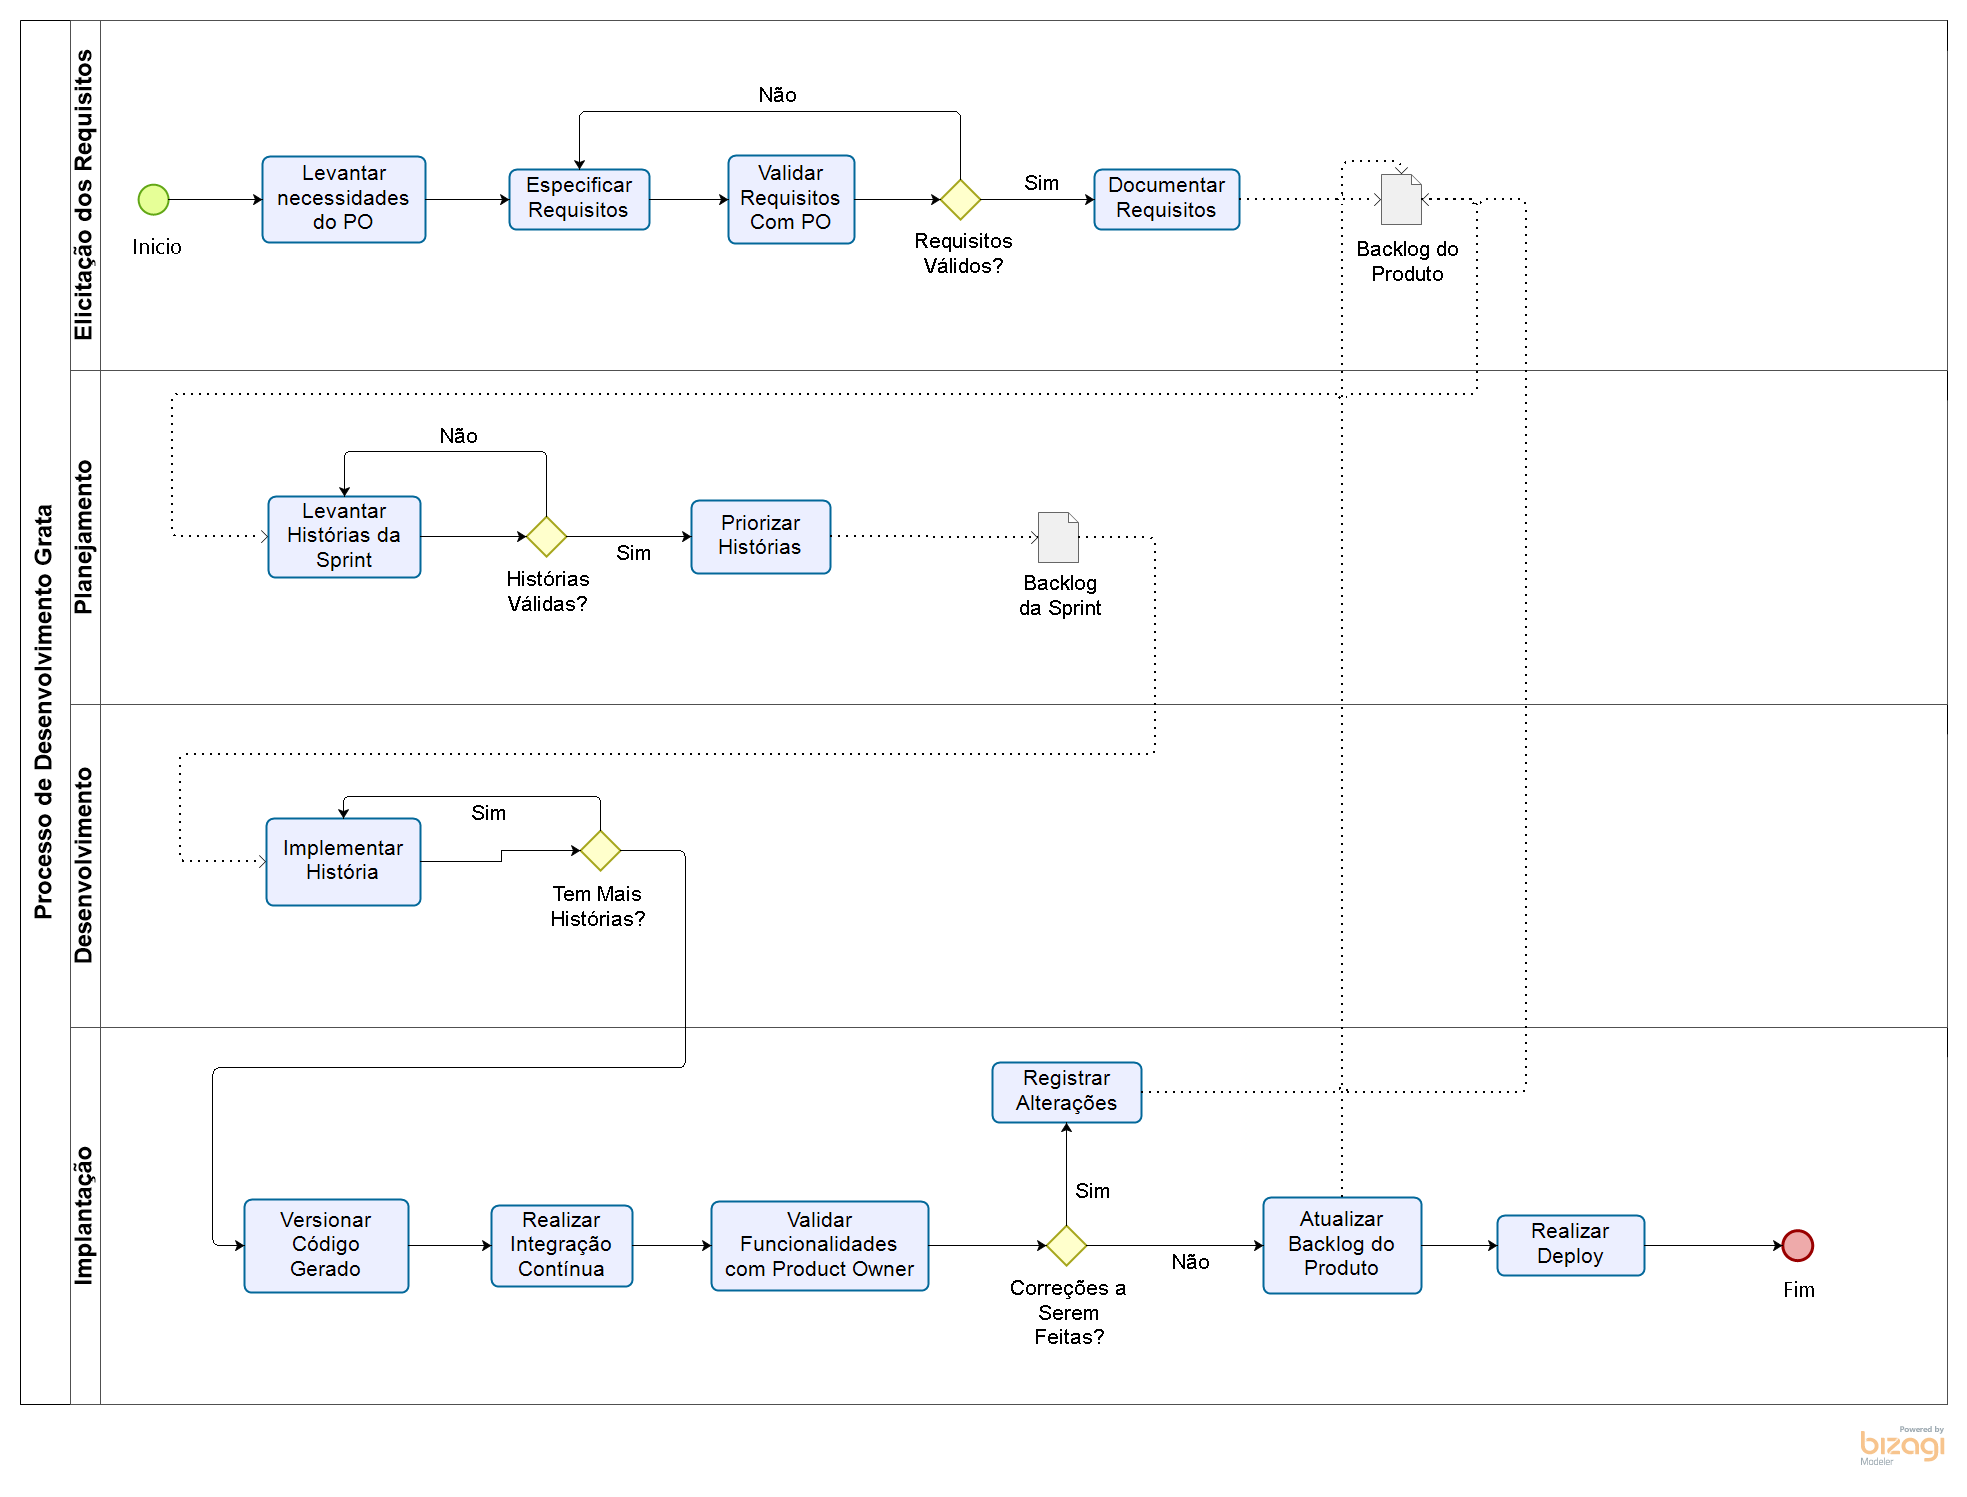
\includegraphics[width=1.0\textwidth]{figuras/processo_de_desenvolvimento.png}
	\caption{Processo de Desenvolvimento do Grata. Fonte: Própria}
	\label{img:processo_de_desenvolvimento}
\end{figure}

\section{Elicitação dos Requisitos}

De acordo com a Figura \ref{img:processo_de_desenvolvimento}, a primeira atividade a ser realizada é elicitação dos requisitos, definidos no tópico \ref{sec:elicitacao_requisitos}. As técnicas utilizadas para elicitação dos requisitos foram entrevista e observação, definidas respectivamente nos tópicos \ref{sec:entrevista} e \ref{sec:observacao}. 

A primeira atividade do processo \ref{img:processo_de_desenvolvimento} foi facilitada pois o desenvolvedor deste projeto estagia no setor do estudo de caso, NMIL, e com isso foram realizadas entrevistas a fim de entender como funciona todo o processo de marcar uma reunião até ela ser realizada. As entrevistas foram do tipo informal, pois assim foi possível entender melhor o contexto inserido. Esses processos podem ser visualizados nas Figuras \ref{img:modelagemProcessoGeral1Parte1}, \ref{img:modelagemProcessoGeral1Parte2}, \ref{img:modelagemProcessoGeral2Parte1} e \ref{img:modelagemProcessoGeral2Parte2}, que juntam englobam todo o processo do setor envolvendo reuniões, que conta com a presença de diversos participantes de diferentes setores.

Após realizar as entrevistas, foram realizadas observações sobre como os \textit{stakeholders} interagem com o sistema em vigor, e foi constatado que o sistema atual chamado Gertiq (Gerenciador de Tíquetes), ele é usado para marcar reuniões, contudo os participantes são chamados via email pela ferramenta \textit{Outlook}, não possuem um sistema para anotar as pautas e atas das reuniões, sendo feitas hoje a partir de folhas de papel.

\subsection{Requisitos Funcionais}

Para a elaboração dos requisitos funcionais, foi constatado a necessidade de uma identificação e descrição dos usuários do sistema, sendo apresentadas a seguir nas Tabelas \ref{tab:usuario_administrador} e \ref{tab:usuario_participante}: 

\begin{table}[H]
	\begin{tabular}{|p{3.0cm}|p{12.0cm}|} 
	\hline
	\textbf{Usuário} & \textbf{Administrador} \\ \hline
	\textbf{Descrição} & Usuário que irá ter total controle sobre o sistema e todas as funcionalidades.  \\ \hline
	\textbf{O que ele faz?} & Ele é responsável pela condução das reuniões, documentar as ATAs, apresentar relatórios e pauta das reuniões, acompanhar a evolução dos projetos, e receber \textit{feedbacks} sobre as reuniões. \\ \hline
	\textbf{O que ele precisa?} & Ele precisa de login e senha para conseguir acessar o sistema. visualizar um ambiente completo com todas as funcionalidades disponíveis no sistema. \\ \hline
	\end{tabular}
	 \caption{Usuário Administrador}
	 \label{tab:usuario_administrador}
\end{table}

\begin{table}[H]
	\begin{tabular}{|p{3.0cm}|p{12.0cm}|} 
	\hline
	\textbf{Usuário} & \textbf{Participante das Reunioes} \\ \hline
	\textbf{Descrição} & Usuário que irá acessar o sistema para visualizar a ATA das reuniões que participou. \\ \hline
	\textbf{O que ele faz?} & Contribui com informações nas reuniões usadas para gerar requisitos do produto. \\ \hline
	\textbf{O que ele precisa?} & Precisa de login e senha para conseguir acessar o sistema, visualizar as ATAas das reunioes que participou, podendo imprimir, baixar, e deixar comentários. \\ \hline
	\end{tabular}
	 \caption{Usuário Participante}
	 \label{tab:usuario_participante}
\end{table}

Após identificados e descritos os usuários do sistema, foi elaborado um diagrama de caso de uso, explicado no tópico \ref{sec:casos_de_uso}, sendo apresentado a seguir:

\begin{figure}[H]
	\centering
	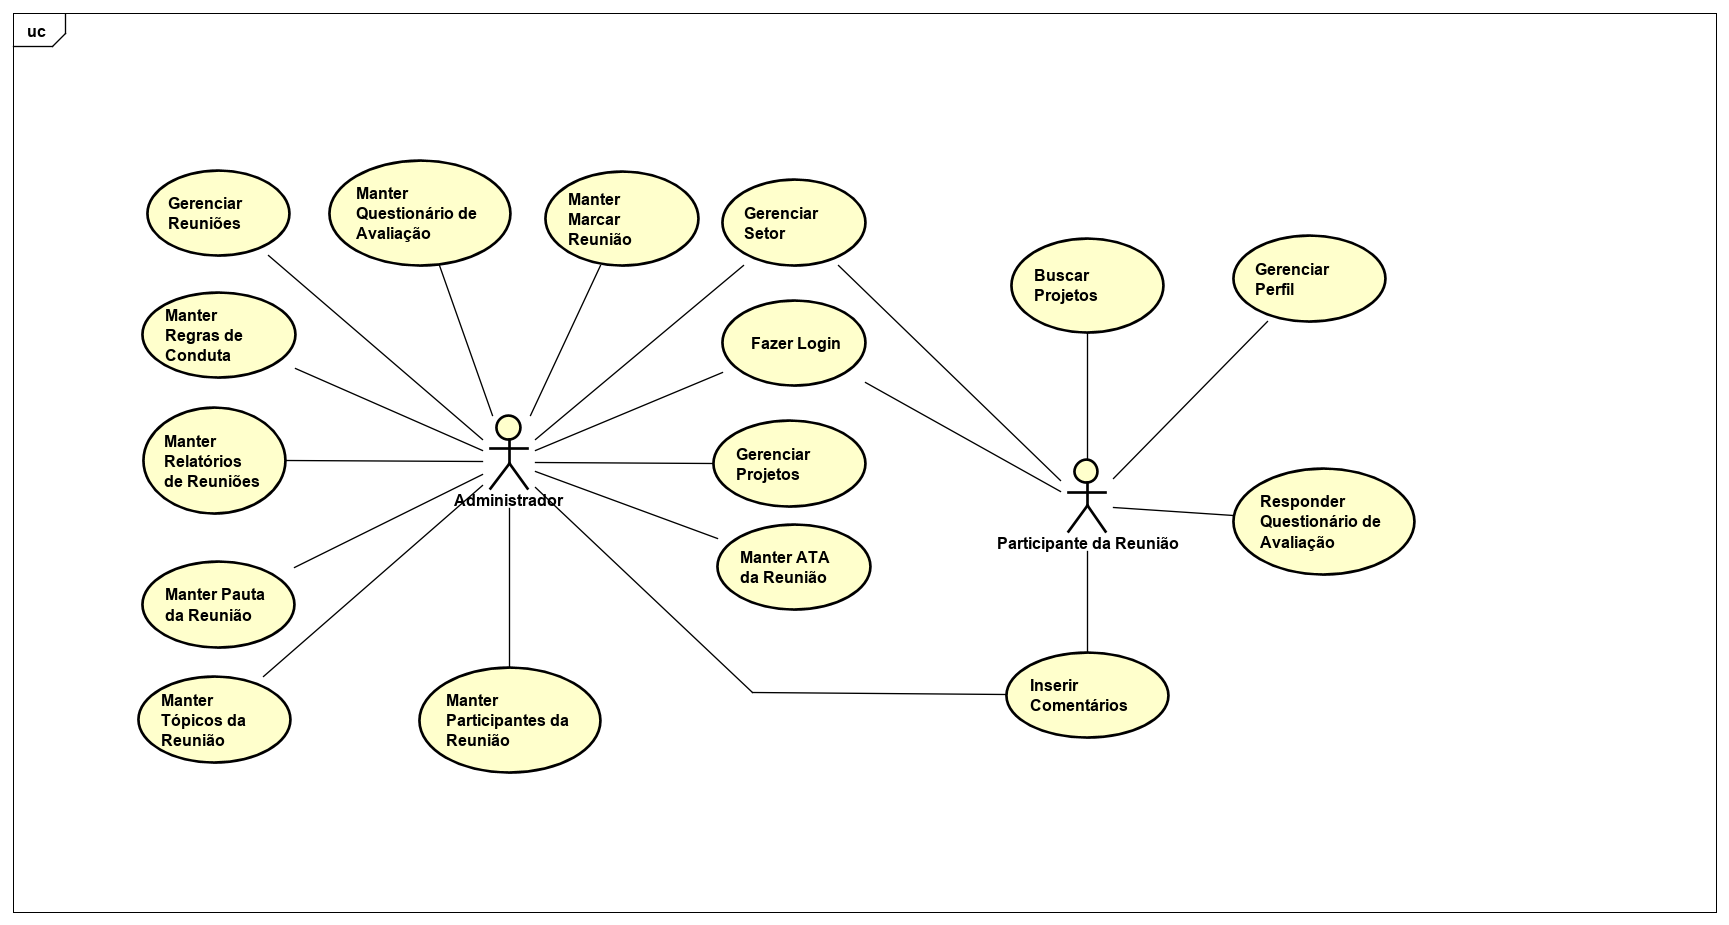
\includegraphics[width=1.0\textwidth]{figuras/casosDeUso.png}
	\caption{Casos de Uso Grata. Fonte: Própria}
	\label{img:casos_de_uso_grata}
\end{figure}

O diagrama de casos de uso da Figura \ref{img:casos_de_uso_grata} foi elaborado não apenas para visualização das funcionalidades, bem como as interações dos atores com o sistema, mas desenvolvido também como auxílio visual das funcionalidades para montar o \textit{backlog} do produto.

\subsubsection{Backlog do Produto}

O Backlog do Produto é composto pelas Histórias de Usuário e Histórias técnicas
elicitadas e desenvolvidas durante as Sprints. Estas representam necessidades levantadas reais para a aplicação, levantadas pelo PO e desenvolvedor.

\subsubsection{Histórias de Usuário}

Nas Tabelas \ref{tab:historias_de_usuario_administrador_parte1}, \ref{tab:historias_de_usuario_administrador_parte2} são apresentadas as Histórias de Usuário elicitadas a partir da análise do diagrama de casos de uso da Figura \ref{img:casos_de_uso_grata}. 
As Histórias de Usuário representam as necessidades levantadas pelo usuário, que culminam em funcionalidades da aplicação. 

\begin{table}[H]
	\begin{tabular}{|p{4.0cm}|p{11.0cm}|} 
	\hline
	\textbf{Funcionalidade} & \textbf{História de Usuário} \\ \hline
	Fazer Login & Eu, como Administrador, desejo poder realizar login, para assim poder acessar as funcionalidades do sistema.  \\ \hline
	Cadastrar Plano de Reuniões & Eu, como Administrador, desejo poder criar, editar, excluir o plano de reuniões, para assim conseguir melhor conduzir as reuniões.\\ \hline
	& Eu, como Administrador, desejo que o sistema converta o plano de reuniões em PDF, para que seja usado mais tarde ao comunicar os participantes da reunião. \\ \hline
	& Eu, como Administrador, desejo que apenas eu possa gerenciar o plano de reuniões, para assim ter total controle sobre a reunião. \\ \hline
	Cadastrar Pauta da Reunião & Eu, como Administrador, desejo poder criar, editar e excluir a pauta da reunião, para assim conseguir ser mais objetivo na reunião. \\ \hline
	& Eu, como Administrador, desejo que quando a reunião estiver com o status "Finalizada", o sistema impeça que as pautas sejam excluídas ou alteradas. \\ \hline
	& Eu, como Administrador, desejo que o sistema converta a pauta da reunião em PDF, para que seja usada mais tarde ao comunicar os participantes da reunião. \\ \hline
	Gerenciar Tópicos da Reunião & Eu, como Administrador, desejo poder criar, editar e excluir os tópicos da reunião, para assim ser mais objetivo com o desenvolvimento da reunião. 
	\\ \hline
	& Eu, como Administrador, desejo que os tópicos criados possam ser adicionados a pauta das reuniões. \\ \hline
	& Eu, como Administrador, desejo que os tópicos sejam tanto adicionados as reuniões, quanto fiquem disponíveis fora delas para que sejam usados em futuras reuniões. \\ \hline
	Gerenciar Regras de Conduta & Eu, como Administrador, desejo poder criar, editar e excluir as regras de conduta, para que assim a reunião não tenha dispersões de foco. \\ \hline
	& Eu, como Administrador, desejo que as regras de conduta criadas possam ser adicionadas a pauta das reuniões. \\ \hline
	& Eu, como Administrador, desejo que as regras de conduta sejam tanta adicionadas as reuniões, quanto fiquem disponíveis foram delas para que sejam usadas em futuras reuniões. \\ \hline
	\end{tabular}
	 \caption{Histórias de Usuário Administrador Parte 1}
	 \label{tab:historias_de_usuario_administrador_parte1}
\end{table}

\begin{table}[H]
	\begin{tabular}{|p{4.0cm}|p{11.0cm}|} 
	\hline
	\textbf{Funcionalidade} & \textbf{História de Usuário} \\ \hline
	Gerar Relatório de Presença & Eu, como Administrador, desejo que o sistema consulte a presença dos participantes. \\ \hline
	& Eu, como Administrador, desejo que o sistema calcule o total de presença dos participantes. \\ \hline
	& Eu, como Administrador, desejo que o sistema exiba o relatório de participantes, contendo a média de presença dos participantes, melhores participantes para se convocar, participantes duvidosos e piores participantes. \\ \hline
	Gerenciar Usuários & Eu, como Administrador, desejo poder criar e excluir usuários do sistema, para assim conseguir ter controle sobre os usuários do sistema. \\ \hline
	& Eu, como Administrador, desejo que apenas eu possa adicionar outros usuário. \\ \hline
	Gerenciar Participantes da Reunião &  Eu, como Administrador, desejo poder adicionar e remover os participantes das reuniões. \\ \hline
	& Eu, como Administrador, desejo que quando a reunião seja marcada, não seja mais possível retirar um participante da reunião. \\ \hline
	& Eu, como Administrador, desejo que ao incluir um participante a reunião, o sistema exporte as informações deste para a ATA. \\ \hline
	Gerenciar Marcar Reunião & Eu, como Administrador, desejo que eu possa incluir, editar e excluir os dados da reunião. \\ \hline
	& Eu, como Administrador, desejo poder visualizar os participantes confirmados ou não à reunião. \\ \hline
	& Eu, como Administrador, desejo que ao marcar reunião, o status da reunião mude para "Agendada" e exiba data e hora. \\ \hline
	& Eu, como Administrador, desejo que caso a reunião seja cancelada, todos os participantes devem receber por \textit{email} a mensagem. \\ \hline
	& Eu, como Administrador, desejo que quando faltar menos que 48 horas para acontecer a reunião, caso ainda não tenha a confirmação de pelo menos 75\% dos convocados, o sistema deve cancelar a reunião \\ \hline
	\end{tabular}
	 \caption{Histórias de Usuário Administrador Parte 2}
	 \label{tab:historias_de_usuario_administrador_parte2}
\end{table}

\begin{table}[H]
	\begin{tabular}{|p{4.0cm}|p{11.0cm}|} 
	\hline
	\textbf{Funcionalidade} & \textbf{História de Usuário} \\ \hline
	Gerar Relatório de Presença & Eu, como Administrador, desejo que o sistema consulte a presença dos participantes. \\ \hline
	& Eu, como Administrador, desejo que o sistema calcule o total de presença dos participantes. \\ \hline 
	\end{tabular}
	 \caption{Histórias de Usuário Administrador Parte 2}
	 \label{tab:historias_de_usuario_administrador_parte3}
\end{table}

% FRONT-END
% A linguagem \textit{front-end} escolhida para este projeto, foi o \textit{React}, pois além de facilitar o desenvolvimento e interação com usuário final, é uma das mais utilizadas ao redor do mundo, então facilita uma manutenção futura e evolução do \textit{software}.


% BACK-END
% A linguagem \textit{back-end} escolhida para este projeto, foi a \textit{Python Django-Rest}, pois tem uma ótima conexão com a linguagem \textit{front-end}, e por ser muito utilizada, possibilitando assim uma manutenção e evolução futura.

%  Neste projeto a arquitetura adotada é uma adaptação ao padrão arquitetural MVC \textit{(model-view-controller)}.



% \subsubsection{Arquitetura do Projeto}

% Neste projeto é feita uma adaptação ao padrão MVC, por conta da escolha da linguagem \textit{front-end}. O \textit{React} possui um padrão arquitetural diferente, chamado de arquitetura de componentes/microserviços. Esse padrão possui semelhanças ao MVC, e o que será utilizado dele será a parte da \textit{View}. Enquanto a linguagem \textit{back-end} é responsável por trabalhar os dados provindos do \textit{front-end} e oferecer um retorno a ele. 

% A seguir será mostrado como funciona separadamente o \textit{React},relacionado ao \textit{front-end} que engloba a \textit{View}, enquanto o \textit{Python Django-Rest} é responsável pelo \textit{back-end} e que engloba a \textit{Model} e a \textit{Controller}:

% \begin{figure}[H]
% 	\centering
% 	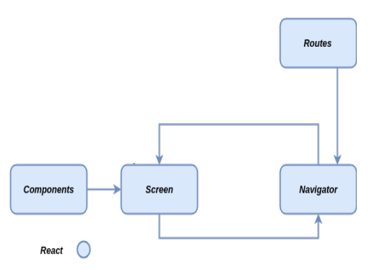
\includegraphics[width=1.0\textwidth]{figuras/diagrama_react.png}
% 	\caption{Diagrama React/Microsserviços}
% 	\label{img:diagrama_react}
% \end{figure}

% \begin{figure}[H]
% 	\centering
% 	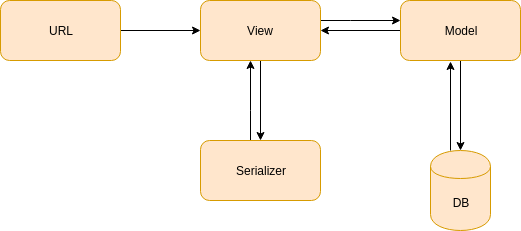
\includegraphics[width=1.0\textwidth]{figuras/django_rest.png}
% 	\caption{Diagrama Django REST Framework}
% 	\label{img:diagrama_rest}
% \end{figure}

% \section{Cronograma TCC}
